\documentclass[11pt,a4paper,oneside]{article}
\usepackage[latin1]{inputenc}
\usepackage{amsmath}
\usepackage{amsfonts}
\usepackage{amssymb}
\usepackage{graphicx}
\usepackage{color}
\usepackage {tikz}
\usepackage{fancyvrb}
\usetikzlibrary {er}
\usepackage[left=2.00cm, right=2.00cm, top=1.00cm]{geometry}
\graphicspath{{./}}
\fvset{tabsize=4}

\begin{document}
	\title{DS 255 - System Virtualization \\ Assignment III - Constructs and Mechanisms for Virtualization}
	\author{Shriram R. \\ M Tech (CDS) \\ 06-02-01-10-51-18-1-15763}
	\maketitle	
	
	\begin{enumerate}
		\item The two mainstream techniques for virtualizing a system are: System VMs and Process VMs. The key differences between the two are described below:
		
		\textbf{System abstraction layer} - System VMs are realized in the ISA/HAL abstraction layer. Process VMs are realized in ABI (application binary interface) abstraction layer or API (Application programming inteface) abstraction layer
		
		\textbf{Shared Resources} - The system VMs share only the execution hardware which includes I/O devices, controllers, MMU, system interconnect (bus) and in some cases CPU cores. Process VMs in addition to execution hardware also share the same OS kernel (drivers + scheduler etc.) and possibly some libraries as well
		
		\textbf{Performance} - System VMs provide better performance as they are manifested in lower abstraction layer. Process VMs are however lightweight in terms of deployment but does not offer good performance compared to System VMs
		
		\textbf{Security} - System VMs provide greater isolation between the guests thereby interference between them is minimized. However, vulnerabilities in the hypervisor can be exploited by the guest code to break the isolation. Process VMs are less secure compared to system VMs in terms of isolation since a fault due to user code in one process can potentially bring down the entire system through kernel panic thereby affecting other process VMs in the same system
		
		\item Emulation is the process of implementing the interface and functionality of one system on another system having a different interface and functionality. It can be used to construct VMs for different ISA scenario by emulating one instruction set on hardware designed for another through techniques like interpretation and binary translation.
		
		Simulation is different from emulation in the sense that it tries to model the environment or functionalities of one system inside software with some approximations and use it run a software designed for that system. Simulation can be used to realize virtual machines although it comes with certain limitations. Some of the key differences are given below,
		
		\begin{center}
			\begin{tabular}{|p{6cm}|p{6cm}|}
				\hline 
				\textbf{Emulation}  & \textbf{Simulation} \\
				\hline
				Emulation can accurately implement a system's functionality and interface & Simulation is just a software model and so can potentially be inaccurate or approximate\\
				\hline
				Emulation can achieve better performance as it generally implemented in a lower abstraction layer and supported by hardware & Simulation has a negative impact on performance as it is generally run inside a computer program which is a higher abstraction layer\\
				\hline 
				Emulation is rigid and quite challenging to continously adapt to change in design & Simulation is a better tool in rapidly adapting to design changes as it is essentially a program \\ 
				\hline
				\end{tabular}
		\end{center}	
		
		\item Virtualization is not exactly the same as abstraction but somewhat similar. Virtualization differs in the sense that it does not necessarily hide details (i.e) the level of detail in a virtual system is often same as that of the real system. While the goal of abstraction is to hide the complexities of one layer in a system from another. However, both virtualization and abstraction provides an additional layer of interface between two existing layers in a system.
		
	    Example: An hard disk is divided into sectors, tracks etc. But an application can read/write files in hard disk without the knowledge of structure of hard disk. This is abstraction where details are hidden. A Virtual machine can perform all kind of operations that it would perform on a real hardware. This is virtualization where the same level of interface / details is available to virtual machine. 
		
		\item \textbf{ISA} - Instruction Set Architecture (ISA) is the interface between hardware and software layer of a system. Application programs and operating system code interact with the hardware through ISA. It is generally divided into user and system ISAs targeted for user applications and OS operations respectively. All System VMs are defined in this layer.
		
		\textbf{ABI} - Application Binary Interface (ABI) provides applications with user instructions (user ISA) and system call interface. The system call interface is used to request privileged functions related to shared hardware etc. Note that the system ISA is not exposed to applications in this interface. Process VMs are defined in this layer.
		
		\textbf{API} - Application Programming Interface (API) provides access to user ISA and standard libraries. Applications can invoke various system services through the library. The API provides an abstraction (sometimes a wrapper) to the implementation of these services. High Level Language (HLL) VMs are defined in this layer. 
		
		\item The challenges in building virtualization support at hardware level are as follows,
			\begin{enumerate}
				\item 
				\item Hardware based ISA translation poses a limitation in code optimization capabilites. Techniques lile inter-instruction optimization, batch optimization are difficult to directly implement in hardware level.
				\item 
				\item 
				\item Virtualizing I/O devices is difficult since it requires additional support from hardware to export these as virtual I/O devices 
			\end{enumerate}
		     The benefits of having virtualization support built in hardware are as follows,
		     \begin{enumerate}
		     	\item Hardware support can remove the need for paravirtualization and can avoid I/O emulation for direct-mapped I/O devices
		     	\item It makes the VM state management simple by allowing the states to be stored in native structures during virtual machine execution
		     	\item Hardare support for Interrupt virtualization in terms of handling external interrupts and interrupt masking greatly simplifies the complexity of VM design
		     	\item Hardware based VMs can provide performance comparable to non-virtualized systems as it avoids the additional software layer for Hypervisor
		     	\item It eliminates the need for shadow page table maintenance used by the hypervisor therefore saving memory. This also reduces memory translation overhead
		     \end{enumerate}		
		
		\item The comparison of emulation, binary translation and para-virtualization in terms of different parameters is given below,
		
		\begin{center}
			\begin{tabular}{|p{2cm}|p{4cm}|p{4cm}|p{4cm}|}
				\hline 
				\textbf{Parameter}  & \textbf{Emulation} & \textbf{Binary Translation} & \textbf{Para-virtualization} \\
				\hline
				Legacy applications & & & \\
				\hline
				Legacy runtime environments & & & Needs modification of guest. So, if the legacy env. is proprietary, then supported is highly limited\\
				\hline
				Application performance & Low translation cost but high execution cost and can affect performance since there is no optimization & High translation cost and low execution cost and can improve performance if the code gets optimized & Overheads of interacting with guest device driver or guest software is reduced. Improves performance of the VM\\
				\hline
			\end{tabular}
		\end{center}
		
		\item \textbf{Different OS - Same ISA} - It is feasible to have para-virtualization. Despite being a different OS, the hypervisor can still modify the guest OS to trap the privileged instructions
		
		\textbf{Same OS - Different ISA} - It is not feasible to have para-virtualization if the ISAs are different. This is because para-virtualization on its own cannot perform emulation or binary translation to convert source to target ISA
		
		\textbf{Different OS - Different ISA} - It is not feasible to have para-virtualization in this case as well. The reason is same as above that the para-virtualization is designed to work on same ISA scenarios with modification to guest OS
		
		\item Desirable characteristics in an ISA for Emulation are as follows,
		      \begin{enumerate}
		      	\item Self-modifying and self-referencing code should not be permitted as it incurs additional challenges and overhead to emulation
		      	\item Stack oriented memory architecture with an abstract memory model if infinite size is desirable as it allows for simple maintenance of program state
		      	\item Indirect jumps should not be permitted as it will cause additional overhead to emulation in terms of finding the code location
		      	\item Precise exception state requirement has to be relaxed and traps should be limited. This means that the exceptions are tested within the program
		      	\item Variable length instructions, padding and mixing of code and data should not be permitted as it poses challenges in code discovery	      	
		      \end{enumerate}
		    
	         %\begin{center}
	         %   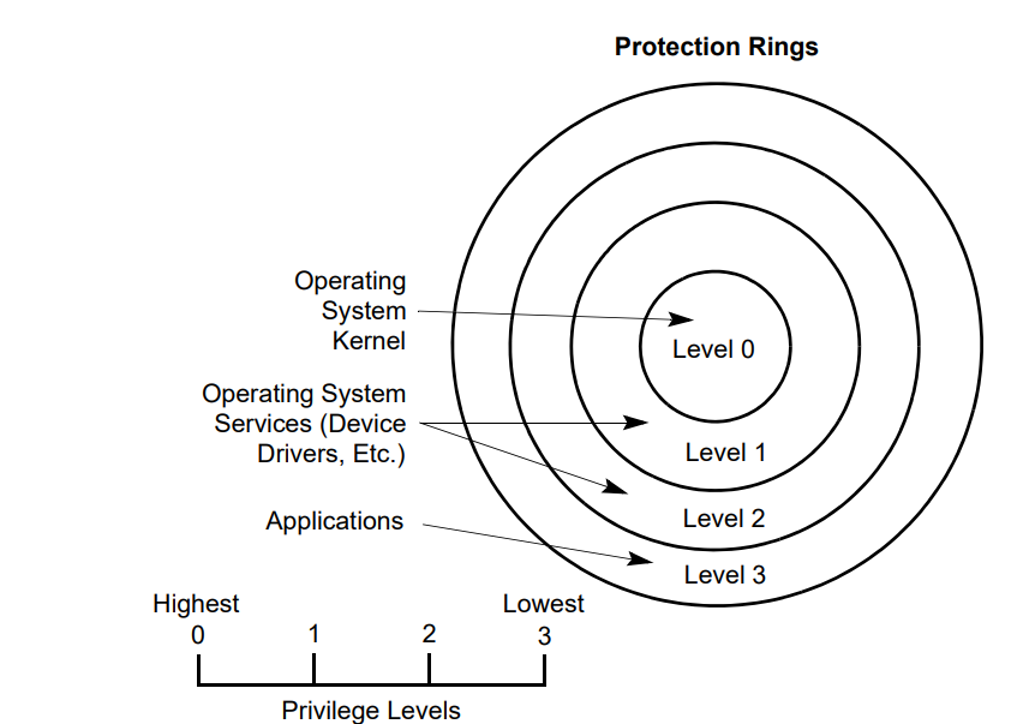
\includegraphics[scale=0.6]{1.png}	[4]
	         %\end{center}			
	\end{enumerate}
    
    \textbf{References}
    \begin{enumerate}
    	\item Jim Smith and Ravi Nair - Virtual Machines: Versatile Platforms for Systems and Processes 
    	\item Course Lecture Notes   	
    \end{enumerate}
 

    
\end{document}